\documentclass[a4paper]{article}

\usepackage[ngerman]{babel}
\usepackage[utf8]{inputenc}
\usepackage{enumitem}
\usepackage{amsmath}
\usepackage{array}
\usepackage{graphicx}
\usepackage{xcolor}


\title{Grundlagen der Rechnerarchitektur\\ Übungsblatt 8\\Gruppe 121\\}
\author{Jonas Otto\and Dominik Authaler}

\date{\today}

\begin{document}

\maketitle

\section*{Aufgabe 1}
\begin{enumerate}[label=\alph*)]
	\item
	\begin{figure}[h!]
		\begin{center}
			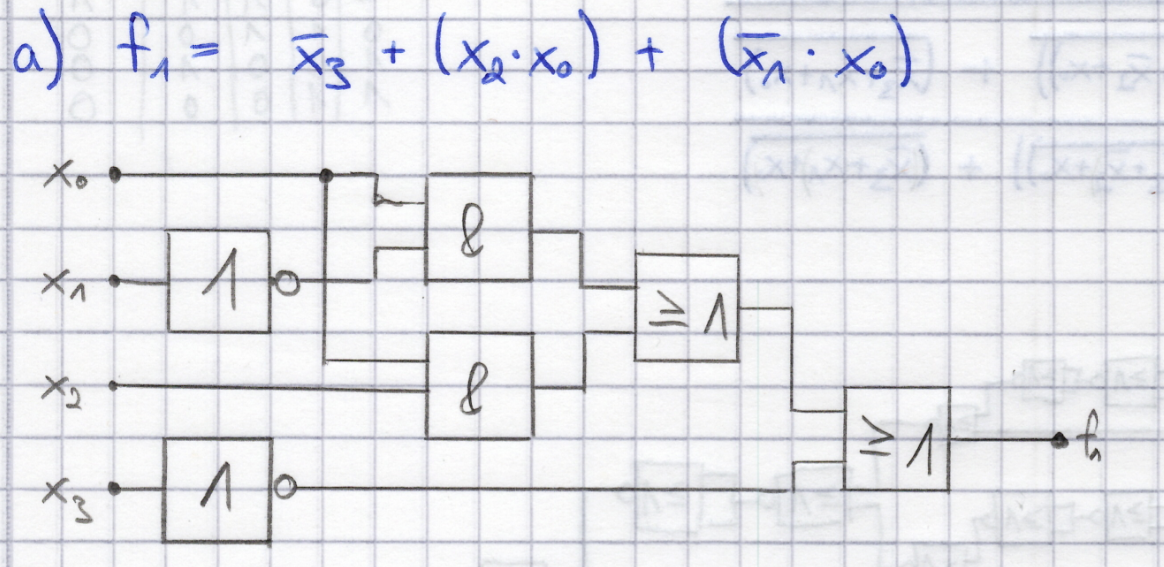
\includegraphics[scale=0.25]{Aufgabe1a.png}
		\end{center}
	\end{figure} 
	\item 
	\begin{figure}[h!]
		\begin{center}
			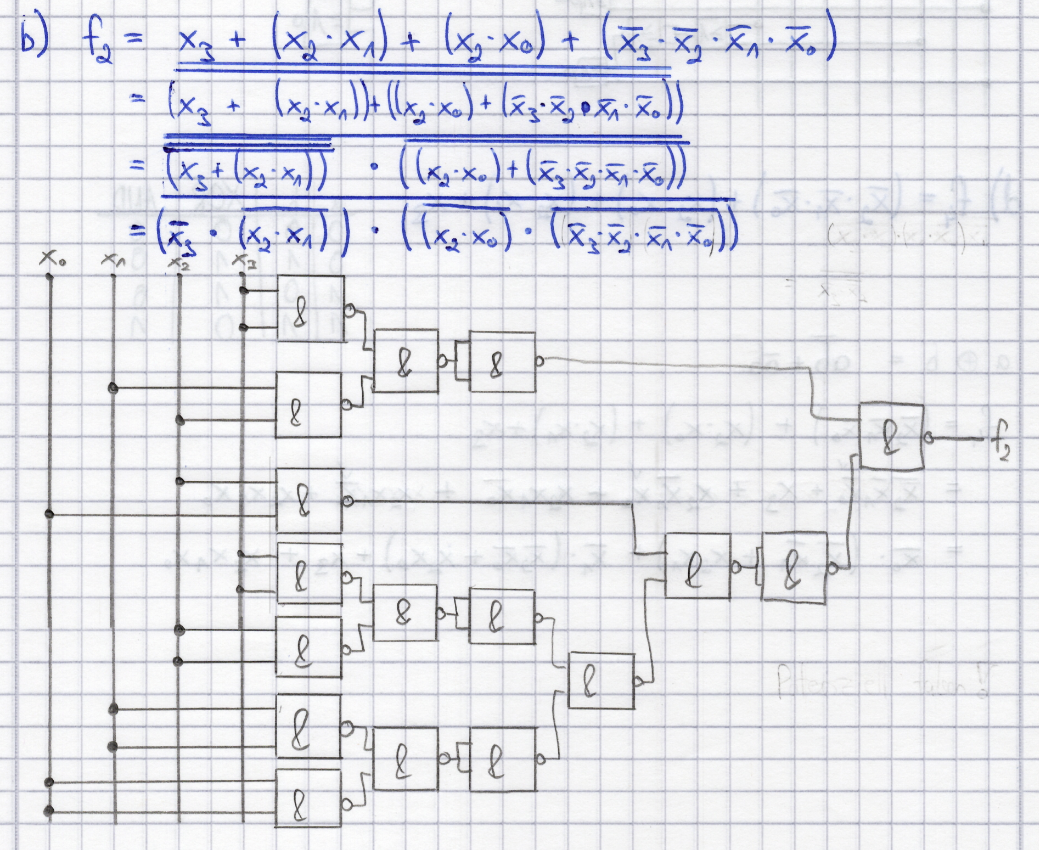
\includegraphics[scale=0.3]{Aufgabe1b.png}
		\end{center}
	\end{figure} 
	\item 
	\begin{figure}[h!]
		\begin{center}
			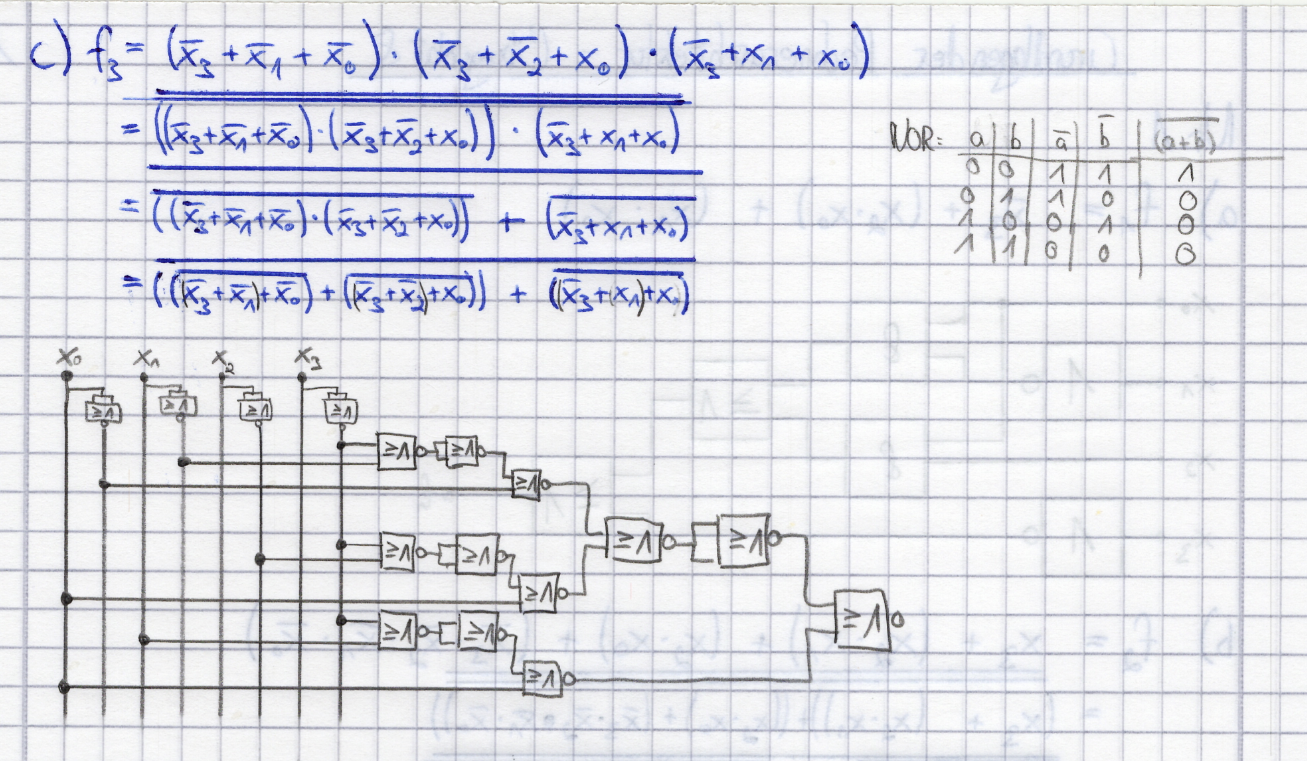
\includegraphics[scale=0.3]{Aufgabe1c.png}
		\end{center}
	\end{figure} 
	\item 
	\begin{align*}
		f_4 &= &(\bar{x}_2 \bar{x}_1 \bar{x}_0) + (x_2x_0) + (x_2x_1) + x_3 \\
			&= &(\bar{x}_1 \cdot \overline{(x_2 + x_0)}) + (x_2x_0) + (x_2x_1) + x_3 \\
			&= &(\bar{x}_1 + (x_2x_0)) \cdot (\overline{(x_2 + x_0)} + (x_2x_0)) + (x_2x_1) + x_3 \\
			&= &(\bar{x}_1 + (x_2x_0)) \cdot (\bar{x}_2\bar{x}_0 + x_2x_0) + (x_2x_1) + x_3 \\
			&= &(\bar{x}_1 + (x_2x_0)) \cdot (\bar{x}_2 \oplus x_0) + (x_2x_1) + x_3 \\
			&= &\overline{(x_1 \cdot \overline{(x_2x_0)})} \cdot (\bar{x}_2 \oplus x_0) + (x_2x_1) + x_3 \\
			&= &\overline{(x_1 \cdot \overline{(x_2x_0)})} \cdot (\bar{x}_2 \oplus x_0) + \overline{(\overline{(x_2x_1)} \cdot \bar{x}_3)} \\
			&= &\overline{\overline{\overline{(x_1 \cdot \overline{(x_2x_0)})} \cdot (\bar{x}_2 \oplus x_0)} \cdot (\overline{(x_2x_1)} \cdot \bar{x}_3)} \\
	\end{align*}
	\begin{figure}[h!]
		\begin{center}
			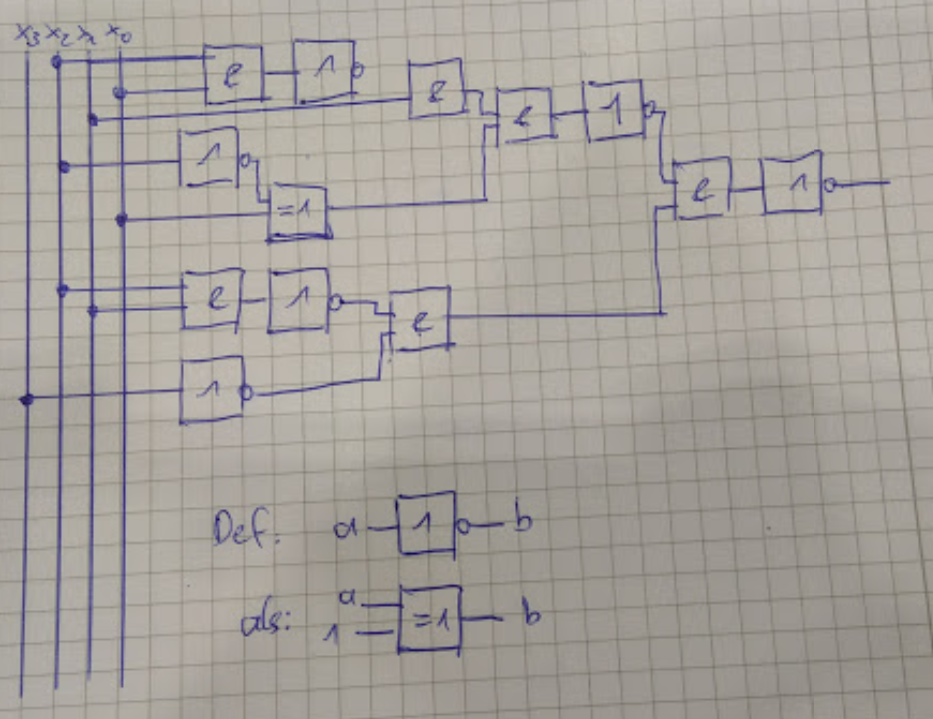
\includegraphics[scale=0.3]{Aufgabe1d.png}
		\end{center}
	\end{figure} 
\end{enumerate}
\section*{Aufgabe 2}
\begin{enumerate}[label=\alph*)]
	\item Wahrheitstabelle: \\
	\begin{tabular}{cccc|c}
		$x_3$ & $x_2$ & $x_1$ & $x_0$ & $f(x)$ \\
		\hline
		0 & 0 & 0 & 0 & 1 \\
		0 & 0 & 0 & 1 & 0 \\
		0 & 0 & 1 & 0 & 0 \\
		0 & 0 & 1 & 1 & 1 \\
		0 & 1 & 0 & 0 & 1 \\
		0 & 1 & 0 & 1 & 0 \\
		0 & 1 & 1 & 0 & 1 \\
		0 & 1 & 1 & 1 & 0 \\
		1 & 0 & 0 & 0 & 1 \\
		1 & 0 & 0 & 1 & 1 \\
		1 & 0 & 1 & 0 & 0 \\
		1 & 0 & 1 & 1 & 0 \\
		1 & 1 & 0 & 0 & 1 \\
		1 & 1 & 0 & 1 & 0 \\
		1 & 1 & 1 & 0 & 0 \\
		1 & 1 & 1 & 1 & 1 \\
	\end{tabular}
	\item
	\begin{equation*}
		f_{DKNF} = \bar{x}_3\bar{x}_2\bar{x}_1\bar{x}_0 + \bar{x}_3\bar{x}_2x_1x_0 + \bar{x}_3 x_2 \bar{x}_1\bar{x}_0 + \bar{x}_3x_2x_1\bar{x}_0 + x_3\bar{x}_2\bar{x}_1\bar{x}_0 + x_3\bar{x}_2\bar{x}_1x_0 + x_3x_2\bar{x}_1\bar{x}_0 + x_3x_2x_1x_0
	\end{equation*} 
	
	\item 
	\begin{align*}
	f_{KKNF} =  &(x_3 + x_2 + x_1 + \bar{x}_0) \cdot (x_3 + x_2 + \bar{x}_1 + x_0) \cdot (x_3 + \bar{x}_2 + x_1 + \bar{x}_0) \cdot (x_3 + \bar{x}_2 + \bar{x}_1 + \bar{x}_0) \\ &\cdot (\bar{x}_3 + x_2 + \bar{x}_1 + x_0) \cdot (\bar{x}_3 + x_2 \bar{x}_1 + \bar{x}_0) \cdot (\bar{x}_3 + \bar{x}_2 + x_1 +\bar{x}_0) \\ &\cdot (\bar{x}_3 + \bar{x}_2 + \bar{x}_1 + x_0)
	\end{align*}
	
	\item 
	\begin{figure}[h!]
		\begin{center}
			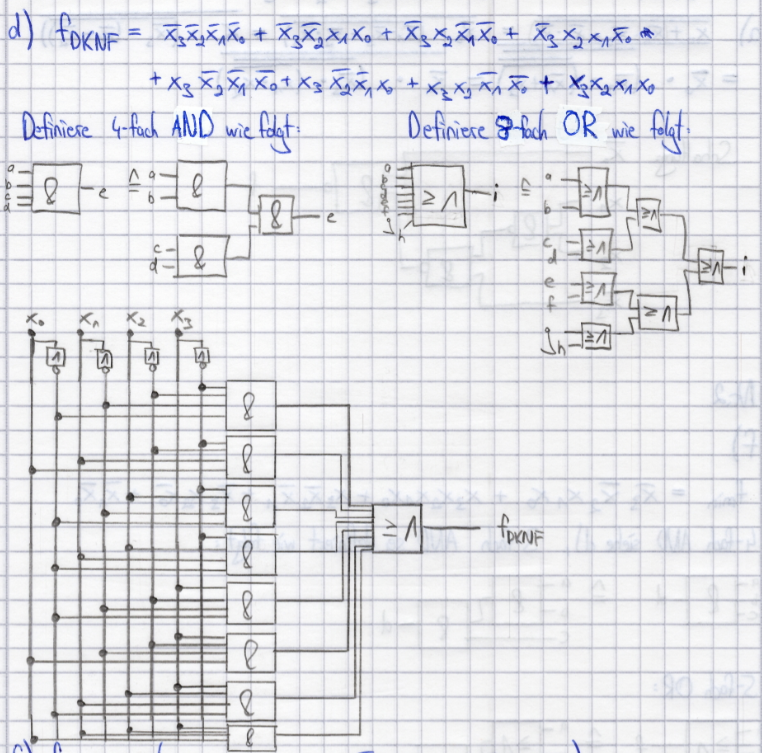
\includegraphics[scale=0.35]{Aufgabe2d.png}
		\end{center}
	\end{figure} 
	
	\item Minimierung mittels KV-Diagrammn:
%	\begin{align*}
%	\begin{array}{c|c|c|c|c|c}
%	&\bar{x}_0&x_0&x_0&\bar{x}_0&\\
%	\hline
%	\bar{x}_1&1&0&0&1&\bar{x}_3\\
%	\hline
%	x_1&0&1&0&1&\bar{x}_3\\
%	\hline
%	x_1&0&0&1&0&x_3\\
%	\hline
%	\bar{x}_1&1&1&0&1&x_3\\
%	\hline
%	&\bar{x}_2&\bar{x}_2&x_2&x_2&\\
%	\end{array}
%	\end{align*}
	
	\begin{figure}[h!]
		\begin{center}
			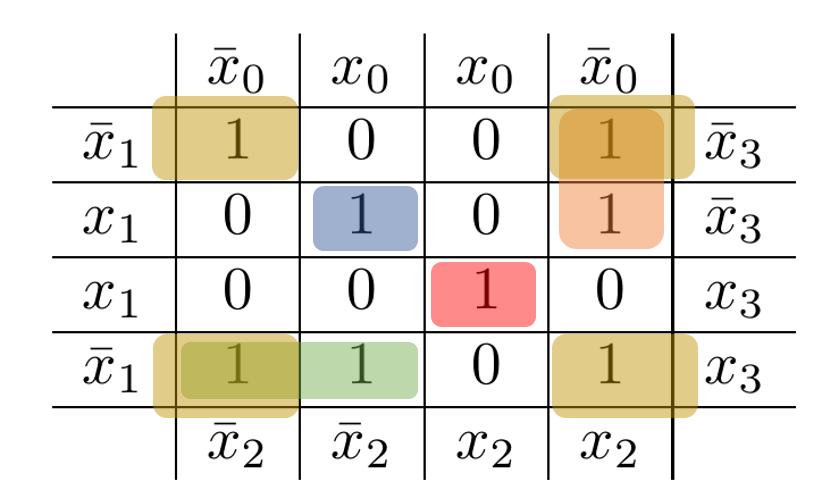
\includegraphics[scale=0.25]{KV_Diagramm.png}
		\end{center}
		\caption{KV-Diagramm zur Minimierung}
	\end{figure}

	\begin{equation*}
	f_{min} = \bar{x}_3\bar{x}_2x_1x_0 + x_3x_2x_1x_0 + x_3\bar{x}_2\bar{x}_1 + \bar{x}_3x_2\bar{x}_0 + \bar{x}_1\bar{x}_0
	\end{equation*} 
	
	\item
	\begin{figure}[h!]
		\begin{center}
			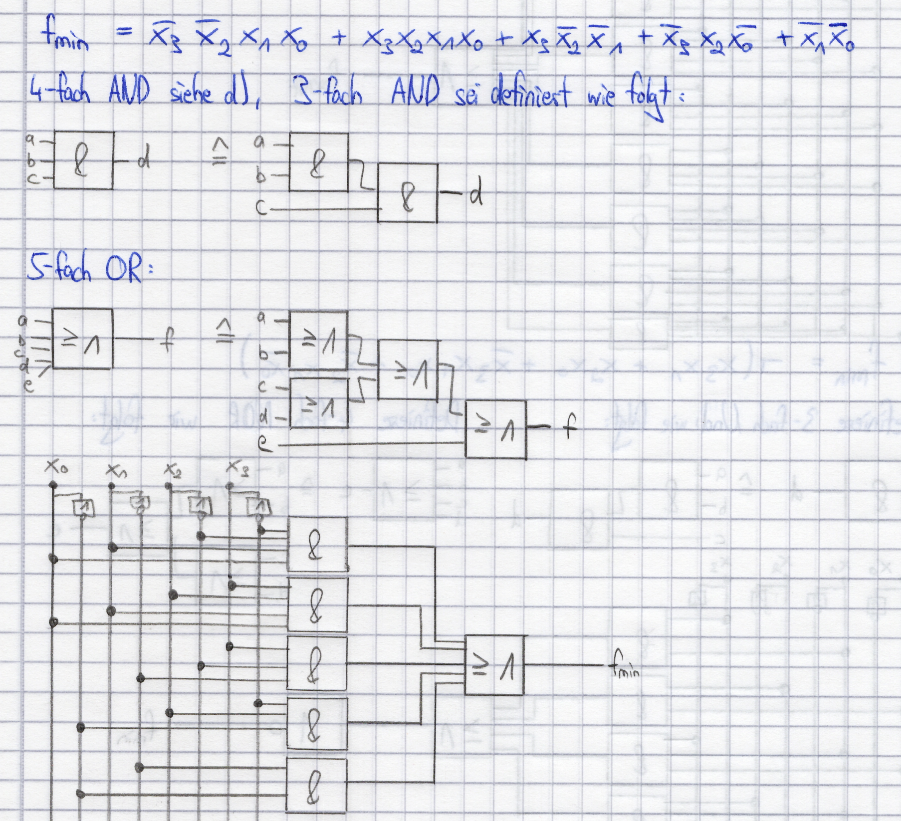
\includegraphics[scale=0.35]{Aufgabe2f.png}
		\end{center}
	\end{figure} 

\end{enumerate}
\section*{Aufgabe 3}
\begin{enumerate}[label=\alph*)]
	\item 
	\begin{align*}
		f &= &x_0 + \bar{x}_1\cdot\bar{x}_3 + \bar{x}_2 \cdot \bar{x}_3 \\
		&= &\overline{\overline{x_0 + (\bar{x}_1\cdot\bar{x}_3 + \bar{x}_2 \cdot \bar{x}_3)}} \\
		&= &\overline{\bar{x}_0 \cdot \overline{(\bar{x}_1\cdot\bar{x}_3 + \bar{x}_2 \cdot \bar{x}_3)}} \\
		&= &\overline{\bar{x}_0 \cdot (\overline{\bar{x}_3 \cdot (\bar{x}_1 + \bar{x}_2)}}) \\
		&= &\overline{\bar{x}_0 \cdot (\overline{\bar{x}_3 \cdot \overline{\overline{(\bar{x}_1 + \bar{x}_2)}}}}) \\
		&= &\overline{\bar{x}_0 \cdot (\overline{\bar{x}_3 \cdot \overline{(x_1 \cdot x_2)}}})
	\end{align*}
	\item \begin{figure}[h!]
		\begin{center}
			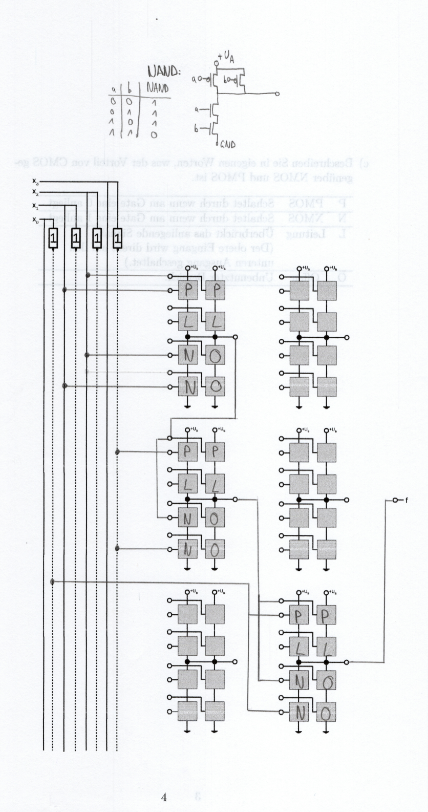
\includegraphics[scale=0.8]{Aufgabe3b.png}
		\end{center}
	\end{figure} 
	\item Bei CMOS Schaltungen (C für complementary) werden NMOS und PMOS Transistoren gezielt kombiniert, um die Verlustleistung der Schaltung zu verringern und damit ihre Energieeffizienz zu steigern. Dabei wird ausgenutzt, dass die beiden Transistortypen ein komplementäres Schaltungsverhalten aufweisen. Wird der Signalausgang einer Schaltung mit einer der beiden Versorgungsschienen (VCC bzw. GND) verbunden, so wird in der CMOS Schaltungstechnik dafür gesorgt, dass mittels des komplementären Schaltungsverhaltens die Verbindung zur anderen Versorgungsschiene getrennt wird. 
\end{enumerate}



\end{document}
	
